%==============================================================================
%  Options & Trading — A One-Hour Course
%  A ~20-slide Beamer deck: markets, stocks, options, pricing, the Greeks,
%  and risk management through option strategies.
%
%  Compile:  latexmk -pdf options-trading-course.tex
%       or:  pdflatex options-trading-course.tex   (run 2-3x for TikZ)
%
%  Requires a standard TeX Live install with: beamer, tikz, pgfplots,
%  amsmath/mathtools, booktabs, xcolor.  No external theme packages needed.
%==============================================================================
\documentclass[11pt,aspectratio=169]{beamer}

%------------------------------------------------------------------ packages
\usepackage[T1]{fontenc}
\usepackage[utf8]{inputenc}
\usepackage{lmodern}
\usepackage{mathtools}
\usepackage{amssymb}
\usepackage{booktabs}
\usepackage{tikz}
\usepackage{pgfplots}
\pgfplotsset{compat=1.16}
\usetikzlibrary{arrows.meta,decorations.pathreplacing,positioning,calc}

%------------------------------------------------------------------ theme
% A clean, flat, "metropolis-inspired" look built only from stock beamer,
% so it compiles anywhere without installing external theme packages.
\usetheme{default}
\usecolortheme{default}
\useinnertheme{default}
\setbeamertemplate{navigation symbols}{}   % remove nav clutter
\setbeamertemplate{itemize items}[circle]
\setbeamertemplate{enumerate items}[default]

% Palette --------------------------------------------------------------------
\definecolor{ink}{HTML}{22303F}      % near-black slate for text
\definecolor{accent}{HTML}{1F6FEB}   % primary blue
\definecolor{accent2}{HTML}{E8590C}  % orange for "the other side" of a trade
\definecolor{good}{HTML}{2F9E44}     % green (profit)
\definecolor{bad}{HTML}{E03131}      % red (loss)
\definecolor{soft}{HTML}{F4F6F8}     % light panel background
\definecolor{muted}{HTML}{6B7A8D}    % secondary text

\setbeamercolor{normal text}{fg=ink}
\setbeamercolor{structure}{fg=accent}
\setbeamercolor{frametitle}{fg=ink}
\setbeamercolor{title}{fg=ink}
\setbeamercolor{alerted text}{fg=accent2}
\setbeamerfont{frametitle}{series=\bfseries,size=\Large}
\setbeamerfont{title}{series=\bfseries,size=\huge}
\setbeamerfont{frametitle}{series=\bfseries}

% Frame title: title text + a thin accent rule underneath ---------------------
\setbeamertemplate{frametitle}{%
  \vspace{0.6em}%
  \usebeamerfont{frametitle}\usebeamercolor[fg]{frametitle}\insertframetitle%
  \vspace{0.2em}\par
  {\color{accent}\rule{\textwidth}{1.2pt}}%
}

% Footline: section . page ----------------------------------------------------
\setbeamertemplate{footline}{%
  \hbox{\begin{beamercolorbox}[wd=\paperwidth,ht=2.6ex,dp=1.2ex,leftskip=1.2em,rightskip=1.2em]{}%
    {\footnotesize\color{muted}\insertshorttitle}\hfill
    {\footnotesize\color{muted}\insertframenumber/\inserttotalframenumber}%
  \end{beamercolorbox}}%
}

%------------------------------------------------------------------ macros
\newcommand{\E}{\mathbb{E}}                 % expectation
\newcommand{\Prob}{\mathbb{P}}              % probability
\newcommand{\Var}{\operatorname{Var}}
\newcommand{\dd}{\mathrm{d}}                % differential
\newcommand{\Ncdf}{\mathrm{N}}             % standard normal CDF
\newcommand{\call}{C}
\newcommand{\putt}{P}
\newcommand{\strike}{K}
\newcommand{\und}{S}                         % underlying price

% Little coloured "key idea" callout box
\newcommand{\keybox}[1]{%
  \begin{beamercolorbox}[wd=\textwidth,sep=0.6em,rounded=true]{}%
    \colorbox{soft}{\parbox{\dimexpr\textwidth-1.4em}{\color{ink}#1}}%
  \end{beamercolorbox}}

% pgfplots default styling for payoff/price charts ----------------------------
\pgfplotsset{
  payoffaxis/.style={
    width=6.4cm, height=4.6cm,
    axis lines=middle,
    axis line style={-{Latex[length=2mm]}, draw=muted},
    tick style={draw=none},
    xlabel style={at={(current axis.right of origin)}, anchor=north west, font=\scriptsize},
    ylabel style={at={(current axis.above origin)}, anchor=south east, font=\scriptsize},
    label style={font=\scriptsize},
    ticklabel style={font=\tiny, color=muted},
    every axis plot/.append style={line width=1.1pt},
    clip=false,
  }
}

\title[Options \& Trading]{Options \& Trading}
\subtitle{Markets, Option Products, the Greeks, and Managing Risk}
\author{}
\date{}

%==============================================================================
\begin{document}

%--- 1. Title ---------------------------------------------------------------
\begin{frame}[plain]
  \vspace{1.2em}
  \begin{center}
    {\color{accent}\rule{0.6\textwidth}{1.4pt}}\\[0.9em]
    {\usebeamerfont{title}\usebeamercolor[fg]{title}\inserttitle}\\[0.5em]
    {\large\color{muted}\insertsubtitle}\\[1.1em]
    {\color{accent}\rule{0.6\textwidth}{1.4pt}}
  \end{center}
  \vfill
  \begin{center}
    \small\color{muted}A one-hour introduction \;$\cdot$\; formal enough to be precise, light enough to follow
  \end{center}
  \vspace{1.0em}
\end{frame}

%--- 2. Roadmap -------------------------------------------------------------
\begin{frame}{What we will cover}
  \begin{columns}[T]
    \begin{column}{0.48\textwidth}
      \textbf{\color{accent}Part I — Foundations}
      \begin{enumerate}
        \item What trading is, and who trades
        \item Stocks and the price process
        \item Risk, return, and volatility
      \end{enumerate}
      \vspace{0.8em}
      \textbf{\color{accent}Part II — Options}
      \begin{enumerate}\setcounter{enumi}{3}
        \item Calls, puts, and payoffs
        \item What an option is worth
        \item Black–Scholes in one slide
      \end{enumerate}
    \end{column}
    \begin{column}{0.48\textwidth}
      \textbf{\color{accent}Part III — The Greeks}
      \begin{enumerate}\setcounter{enumi}{6}
        \item Delta and hedging
        \item Gamma, Theta, Vega
        \item Implied volatility \& the smile
      \end{enumerate}
      \vspace{0.8em}
      \textbf{\color{accent}Part IV — Strategies \& Risk}
      \begin{enumerate}\setcounter{enumi}{9}
        \item Directional \& volatility strategies
        \item Managing a book with the Greeks
      \end{enumerate}
    \end{column}
  \end{columns}
  \vfill
  \keybox{\textbf{Goal:} understand \emph{why} options exist, \emph{how} they are priced, and \emph{how} they are used to shape and control risk.}
\end{frame}

%--- 3. What is trading -----------------------------------------------------
\begin{frame}{Part I — What is trading?}
  Trading is the voluntary exchange of a financial asset for cash at an
  agreed price. A \alert{market} is simply the place where buyers and
  sellers meet.
  \vspace{0.6em}
  \begin{columns}[T]
    \begin{column}{0.5\textwidth}
      \textbf{Key quantities}
      \begin{itemize}
        \item \textbf{Bid} — best price a buyer offers
        \item \textbf{Ask} — best price a seller asks
        \item \textbf{Spread} $=\text{Ask}-\text{Bid}$
        \item \textbf{Liquidity} — how easily you trade without moving the price
      \end{itemize}
    \end{column}
    \begin{column}{0.5\textwidth}
      \textbf{Why people trade}
      \begin{itemize}
        \item \textbf{Investing} — own a claim on future cash flows
        \item \textbf{Hedging} — reduce an existing risk
        \item \textbf{Speculation} — take a view on the price
        \item \textbf{Market-making} — earn the spread by providing liquidity
      \end{itemize}
    \end{column}
  \end{columns}
  \vfill
  \keybox{A trade has \emph{two} sides. Your profit is someone's cost — pricing is about agreeing on a \emph{fair} number.}
\end{frame}

%--- 4. Stocks --------------------------------------------------------------
\begin{frame}{Stocks: a share of a company}
  A \alert{stock} (share) is a unit of ownership in a company. Owning
  $n$ shares of a firm with $N$ shares outstanding entitles you to a
  fraction $n/N$ of its equity, its dividends, and its votes.
  \vspace{0.5em}
  \begin{itemize}
    \item \textbf{Price} $\und_t$ — what one share trades for at time $t$.
    \item \textbf{Market capitalisation} $= N \cdot \und_t$ — the firm's equity value.
    \item \textbf{Dividend} — periodic cash paid to shareholders.
    \item \textbf{Total return} combines price change \emph{and} dividends.
  \end{itemize}
  \vspace{0.4em}
  The price is set continuously by supply and demand. From a trader's
  point of view $\und_t$ is best modelled not as a fixed number but as a
  \alert{random process} — we cannot predict tomorrow's price, only
  describe its distribution.
\end{frame}

%--- 5. The price process ---------------------------------------------------
\begin{frame}{The price as a stochastic process}
  A standard model for a non-dividend stock is \alert{Geometric Brownian
  Motion (GBM)}:
  \[
    \dd \und_t \;=\; \underbrace{\mu\,\und_t\,\dd t}_{\text{drift (trend)}}
      \;+\; \underbrace{\sigma\,\und_t\,\dd W_t}_{\text{diffusion (noise)}},
  \]
  where $W_t$ is Brownian motion, $\mu$ the expected growth rate and
  $\sigma$ the \alert{volatility}. Its solution is log-normal:
  \[
    \und_T \;=\; \und_0 \,\exp\!\Big[\big(\mu-\tfrac12\sigma^2\big)T
      \;+\; \sigma\sqrt{T}\,Z\Big],\qquad Z\sim\Ncdf(0,1).
  \]
  \begin{columns}[c]
    \begin{column}{0.58\textwidth}
      \begin{itemize}
        \item Returns are random; \emph{log}-returns are (roughly) normal.
        \item $\mu$ tilts the average path; $\sigma$ sets its width.
        \item More time $\Rightarrow$ more uncertainty ($\propto\sqrt{T}$).
      \end{itemize}
    \end{column}
    \begin{column}{0.42\textwidth}
      \centering
      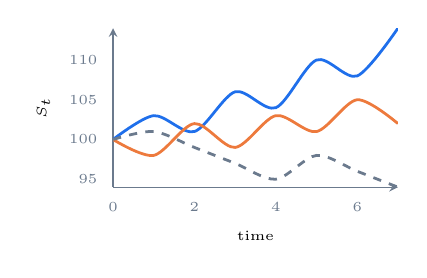
\begin{tikzpicture}
        \begin{axis}[width=5.2cm,height=3.6cm,axis lines=left,
            tick style={draw=none}, ticklabel style={font=\tiny,color=muted},
            xlabel={\tiny time}, ylabel={\tiny $S_t$}, label style={font=\tiny},
            axis line style={draw=muted}]
          \addplot[accent, line width=1pt, smooth]
            coordinates {(0,100)(1,103)(2,101)(3,106)(4,104)(5,110)(6,108)(7,114)};
          \addplot[accent2!80, line width=1pt, smooth]
            coordinates {(0,100)(1,98)(2,102)(3,99)(4,103)(5,101)(6,105)(7,102)};
          \addplot[muted, line width=1pt, smooth, dashed]
            coordinates {(0,100)(1,101)(2,99)(3,97)(4,95)(5,98)(6,96)(7,94)};
        \end{axis}
      \end{tikzpicture}\\
      {\tiny\color{muted}three simulated price paths}
    \end{column}
  \end{columns}
\end{frame}

%--- 6. Risk and return -----------------------------------------------------
\begin{frame}{Risk, return, and volatility}
  Over a horizon, the (log) return is a random variable. We summarise it
  with its first two moments:
  \[
    \text{return } R = \frac{\und_T-\und_0}{\und_0},\qquad
    \mu_R=\E[R]\ (\text{reward}),\qquad
    \sigma_R=\sqrt{\Var[R]}\ (\text{risk}).
  \]
  \begin{columns}[T]
    \begin{column}{0.5\textwidth}
      \begin{itemize}
        \item \textbf{Volatility} $\sigma$ is the standard deviation of returns — the single most important number for options.
        \item It scales with the square root of time: $\sigma_{\text{annual}} = \sigma_{\text{daily}}\sqrt{252}$.
        \item Higher $\sigma$ $\Rightarrow$ wider outcomes $\Rightarrow$ \emph{more valuable} optionality.
      \end{itemize}
    \end{column}
    \begin{column}{0.5\textwidth}
      \centering
      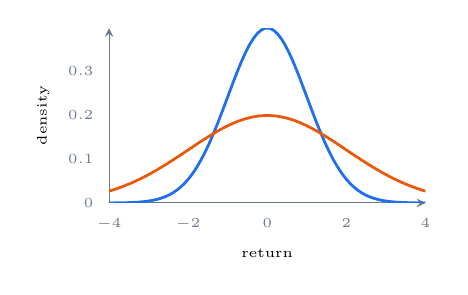
\begin{tikzpicture}
        \begin{axis}[width=5.6cm,height=3.8cm,axis lines=left,
            tick style={draw=none}, ticklabel style={font=\tiny,color=muted},
            xlabel={\tiny return}, ylabel={\tiny density}, label style={font=\tiny},
            axis line style={draw=muted}, domain=-4:4, samples=80]
          \addplot[accent, line width=1pt] {exp(-x^2/2)/sqrt(2*pi)};
          \addplot[accent2, line width=1pt] {exp(-x^2/8)/sqrt(8*pi)};
        \end{axis}
      \end{tikzpicture}\\
      {\tiny\color{muted}low-$\sigma$ (blue) vs.\ high-$\sigma$ (orange)}
    \end{column}
  \end{columns}
  \vspace{0.2em}
  \keybox{Risk is not the enemy — it is the \emph{raw material} options are built from.}
\end{frame}

%--- 7. What is an option ---------------------------------------------------
\begin{frame}{Part II — What is an option?}
  An \alert{option} is a contract giving its holder the \emph{right, but
  not the obligation}, to buy or sell an underlying asset at a fixed
  \alert{strike} price $\strike$ before or at \alert{expiry} $T$.
  \vspace{0.6em}
  \begin{columns}[T]
    \begin{column}{0.5\textwidth}
      \textbf{Call option}
      \begin{itemize}
        \item Right to \textbf{buy} at $\strike$.
        \item Bet that $\und$ will \textbf{rise}.
        \item Payoff at $T$: $\max(\und_T-\strike,\,0)$.
      \end{itemize}
    \end{column}
    \begin{column}{0.5\textwidth}
      \textbf{Put option}
      \begin{itemize}
        \item Right to \textbf{sell} at $\strike$.
        \item Bet that $\und$ will \textbf{fall}.
        \item Payoff at $T$: $\max(\strike-\und_T,\,0)$.
      \end{itemize}
    \end{column}
  \end{columns}
  \vspace{0.5em}
  \begin{itemize}
    \item The buyer pays a \alert{premium} up front for this right.
    \item \textbf{American} options exercise any time up to $T$; \textbf{European} only at $T$.
    \item Every contract has a \textbf{buyer} (long, limited loss) and a \textbf{seller/writer} (short, obligated).
  \end{itemize}
\end{frame}

%--- 8. Payoff diagrams -----------------------------------------------------
\begin{frame}{Payoffs at expiry}
  The value at expiry depends only on where $\und_T$ lands relative to $\strike$.
  \vspace{0.3em}
  \begin{columns}[T]
    \begin{column}{0.25\textwidth}
      \centering{\scriptsize\textbf{Long Call}}\\[-0.2em]
      \begin{tikzpicture}
        \begin{axis}[payoffaxis, xlabel={$S_T$}, ymin=-1.5, ymax=3, xmin=0, xmax=4, xtick={2}, xticklabels={$K$}, ytick=\empty]
          \addplot[good, domain=0:2]{-1};
          \addplot[good, domain=2:4]{-1+(x-2)};
          \draw[muted,dashed] (axis cs:0,0)--(axis cs:4,0);
        \end{axis}
      \end{tikzpicture}
    \end{column}
    \begin{column}{0.25\textwidth}
      \centering{\scriptsize\textbf{Long Put}}\\[-0.2em]
      \begin{tikzpicture}
        \begin{axis}[payoffaxis, xlabel={$S_T$}, ymin=-1.5, ymax=3, xmin=0, xmax=4, xtick={2}, xticklabels={$K$}, ytick=\empty]
          \addplot[good, domain=0:2]{-1+(2-x)};
          \addplot[good, domain=2:4]{-1};
          \draw[muted,dashed] (axis cs:0,0)--(axis cs:4,0);
        \end{axis}
      \end{tikzpicture}
    \end{column}
    \begin{column}{0.25\textwidth}
      \centering{\scriptsize\textbf{Short Call}}\\[-0.2em]
      \begin{tikzpicture}
        \begin{axis}[payoffaxis, xlabel={$S_T$}, ymin=-3, ymax=1.5, xmin=0, xmax=4, xtick={2}, xticklabels={$K$}, ytick=\empty]
          \addplot[bad, domain=0:2]{1};
          \addplot[bad, domain=2:4]{1-(x-2)};
          \draw[muted,dashed] (axis cs:0,0)--(axis cs:4,0);
        \end{axis}
      \end{tikzpicture}
    \end{column}
    \begin{column}{0.25\textwidth}
      \centering{\scriptsize\textbf{Short Put}}\\[-0.2em]
      \begin{tikzpicture}
        \begin{axis}[payoffaxis, xlabel={$S_T$}, ymin=-3, ymax=1.5, xmin=0, xmax=4, xtick={2}, xticklabels={$K$}, ytick=\empty]
          \addplot[bad, domain=0:2]{1-(2-x)};
          \addplot[bad, domain=2:4]{1};
          \draw[muted,dashed] (axis cs:0,0)--(axis cs:4,0);
        \end{axis}
      \end{tikzpicture}
    \end{column}
  \end{columns}
  \vspace{0.2em}
  \begin{itemize}\small
    \item Solid line = payoff \emph{net of premium}; the dashed line is break-even.
    \item Buyers have \textbf{capped loss} (the premium) and \textbf{convex} upside.
    \item Writers collect the premium but carry \textbf{open-ended} risk — the mirror image.
  \end{itemize}
\end{frame}

%--- 9. What an option is worth ---------------------------------------------
\begin{frame}{What is an option worth before expiry?}
  Before expiry, an option's premium splits into two parts:
  \[
    \underbrace{\call_t}_{\text{price}} \;=\;
    \underbrace{\max(\und_t-\strike,0)}_{\text{intrinsic value}}
    \;+\;
    \underbrace{\text{time value}}_{\ \ge 0,\ \text{from future uncertainty}}.
  \]
  \begin{columns}[T]
    \begin{column}{0.54\textwidth}
      \textbf{Moneyness} (for a call):
      \begin{itemize}
        \item \textbf{ITM} — in the money, $\und>\strike$
        \item \textbf{ATM} — at the money, $\und\approx\strike$
        \item \textbf{OTM} — out of the money, $\und<\strike$
      \end{itemize}
      \vspace{0.3em}
      Time value is \emph{largest} at the money and \emph{decays} to zero
      as $t\to T$ (``theta decay'').
    \end{column}
    \begin{column}{0.46\textwidth}
      \centering
      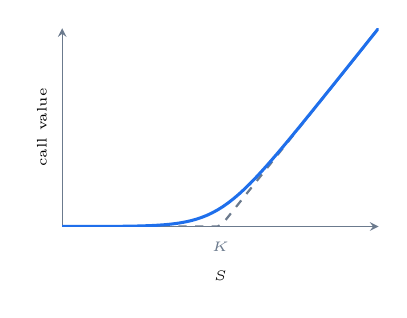
\begin{tikzpicture}
        \begin{axis}[width=5.6cm,height=4.1cm,axis lines=left,
            tick style={draw=none}, xlabel={\tiny $S$}, ylabel={\tiny call value},
            label style={font=\tiny}, ticklabel style={font=\tiny,color=muted},
            axis line style={draw=muted}, xmin=40,xmax=160,ymin=0,ymax=60,
            xtick={100}, xticklabels={$K$}, ytick=\empty, domain=40:160, samples=60]
          \addplot[muted, dashed, line width=0.8pt, domain=40:160]{max(x-100,0)};
          \addplot[accent, line width=1.1pt]{ 8*ln(1+exp((x-100)/8)) };
        \end{axis}
      \end{tikzpicture}\\
      {\tiny\color{muted}price (blue) sits above intrinsic (dashed)}
    \end{column}
  \end{columns}
\end{frame}

%--- 10. Black-Scholes ------------------------------------------------------
\begin{frame}{Black--Scholes in one slide}
  Under GBM with constant volatility $\sigma$ and risk-free rate $r$, the
  fair price of a \emph{European call} is
  \[
    \call \;=\; \und_0\,\Ncdf(d_1)\;-\;\strike\,e^{-rT}\,\Ncdf(d_2),
    \qquad
    d_{1,2}=\frac{\ln(\und_0/\strike)+\big(r\pm\tfrac12\sigma^2\big)T}{\sigma\sqrt{T}} .
  \]
  \begin{columns}[T]
    \begin{column}{0.55\textwidth}
      \textbf{Where it comes from}
      \begin{itemize}\small
        \item Build a portfolio of the option \emph{hedged} with $\Delta$ shares so it is momentarily \textbf{risk-free}.
        \item A risk-free portfolio must earn the risk-free rate $r$ — no free lunch (\alert{no arbitrage}).
        \item That argument becomes a PDE whose solution is the formula above.
      \end{itemize}
    \end{column}
    \begin{column}{0.45\textwidth}
      \textbf{What drives the price}
      \begin{itemize}\small
        \item $\und_0\uparrow \Rightarrow \call\uparrow$
        \item $\strike\uparrow \Rightarrow \call\downarrow$
        \item $\sigma\uparrow \Rightarrow \call\uparrow$ (both calls \& puts!)
        \item $T\uparrow \Rightarrow \call\uparrow$
        \item $r\uparrow \Rightarrow \call\uparrow$
      \end{itemize}
    \end{column}
  \end{columns}
  \vspace{0.2em}
  \keybox{\textbf{Put--call parity:} $\ \call-\putt=\und_0-\strike e^{-rT}$. Calls and puts are two faces of the same coin.}
\end{frame}

%--- 11. The Greeks overview ------------------------------------------------
\begin{frame}{Part III — The Greeks: sensitivities of the price}
  The \alert{Greeks} are the partial derivatives of the option price with
  respect to each input. They tell you \emph{how your P\&L moves} when the
  world moves.
  \vspace{0.4em}
  \begin{center}\small
  \begin{tabular}{@{}l l l l@{}}
    \toprule
    \textbf{Greek} & \textbf{Symbol} & \textbf{Measures sensitivity to} & \textbf{Definition}\\
    \midrule
    Delta & $\Delta$ & underlying price $\und$      & $\partial \call/\partial \und$\\
    Gamma & $\Gamma$ & \emph{change} in Delta        & $\partial^2 \call/\partial \und^2$\\
    Theta & $\Theta$ & passage of time (decay)       & $\partial \call/\partial t$\\
    Vega  & $\mathcal{V}$ & volatility $\sigma$       & $\partial \call/\partial \sigma$\\
    Rho   & $\rho$   & interest rate $r$             & $\partial \call/\partial r$\\
    \bottomrule
  \end{tabular}
  \end{center}
  \vspace{0.3em}
  \keybox{A position's total risk is the \emph{sum} of its Greeks. Manage the book $\Rightarrow$ manage the Greeks.}
\end{frame}

%--- 12. Delta --------------------------------------------------------------
\begin{frame}{Delta: exposure to the underlying}
  \[
    \Delta \;=\; \frac{\partial \call}{\partial \und} \;=\; \Ncdf(d_1)\ \in[0,1]\ \text{for a call},\qquad
    \Delta_{\putt}=\Ncdf(d_1)-1\ \in[-1,0].
  \]
  \begin{columns}[c]
    \begin{column}{0.55\textwidth}
      \textbf{Three readings of Delta}
      \begin{itemize}\small
        \item \textbf{Slope:} how much the option gains if $\und$ rises by \$1.
        \item \textbf{Equivalent shares:} a $\Delta=0.6$ call behaves like holding $0.6$ shares.
        \item \textbf{Risk-neutral probability} (roughly) that the option finishes in the money.
      \end{itemize}
      \vspace{0.3em}
      Deep ITM call $\Delta\!\to\!1$; deep OTM $\Delta\!\to\!0$; ATM $\Delta\!\approx\!0.5$.
    \end{column}
    \begin{column}{0.45\textwidth}
      \centering
      \begin{tikzpicture}
        \begin{axis}[width=5.6cm,height=4.1cm,axis lines=left,
            tick style={draw=none}, xlabel={\tiny $S$}, ylabel={\tiny $\Delta$ (call)},
            label style={font=\tiny}, ticklabel style={font=\tiny,color=muted},
            axis line style={draw=muted}, xmin=40,xmax=160,ymin=0,ymax=1.05,
            xtick={100}, xticklabels={$K$}, ytick={0,0.5,1},
            domain=40:160, samples=80]
          \addplot[accent, line width=1.1pt]{ 1/(1+exp(-(x-100)/12)) };
          \draw[muted,dashed] (axis cs:100,0)--(axis cs:100,0.5);
        \end{axis}
      \end{tikzpicture}\\
      {\tiny\color{muted}Delta runs smoothly from 0 to 1}
    \end{column}
  \end{columns}
\end{frame}

%--- 13. Delta hedging ------------------------------------------------------
\begin{frame}{Delta hedging: turning options into a risk-free recipe}
  To neutralise price risk, hold $\Delta$ shares \emph{short} against a long
  call. The combined position is \alert{delta-neutral}: to first order it
  does not move when $\und$ moves.
  \[
    \Pi \;=\; \call - \Delta\,\und
    \qquad\Longrightarrow\qquad
    \frac{\partial \Pi}{\partial \und}=0 .
  \]
  \begin{itemize}
    \item As $\und$ moves, $\Delta$ changes (that is Gamma), so the hedge must be \alert{rebalanced} — this is \textbf{dynamic hedging}.
    \item Continuously rebalancing \emph{replicates} the option: this is exactly the Black--Scholes argument in action.
    \item In practice you rebalance discretely; the mismatch is the cost/benefit of \textbf{Gamma}.
  \end{itemize}
  \vspace{0.2em}
  \keybox{Market-makers quote options and then \emph{delta-hedge} — they want the spread, not a directional bet.}
\end{frame}

%--- 14. Gamma, Theta, Vega -------------------------------------------------
\begin{frame}{Gamma, Theta, Vega — the second-order picture}
  \begin{columns}[T]
    \begin{column}{0.33\textwidth}
      \textbf{\color{accent}Gamma $\Gamma$}
      \begin{itemize}\small
        \item Curvature of value; how fast $\Delta$ moves.
        \item \textbf{Long} options $\Rightarrow$ long Gamma: you profit from big moves.
        \item Peaks \textbf{at the money}, near expiry.
      \end{itemize}
    \end{column}
    \begin{column}{0.33\textwidth}
      \textbf{\color{accent}Theta $\Theta$}
      \begin{itemize}\small
        \item Time decay: value lost per day, all else equal.
        \item Long options \textbf{pay} Theta; short options \textbf{earn} it.
        \item The price of holding convexity.
      \end{itemize}
    \end{column}
    \begin{column}{0.33\textwidth}
      \textbf{\color{accent}Vega $\mathcal{V}$}
      \begin{itemize}\small
        \item Sensitivity to volatility $\sigma$.
        \item Long options are \textbf{long Vega}: gain if vol rises.
        \item Largest for longer-dated, ATM options.
      \end{itemize}
    \end{column}
  \end{columns}
  \vspace{0.6em}
  \keybox{\textbf{The fundamental trade-off:} being long options gives you Gamma and Vega, but you \emph{pay} Theta every day. Being short flips all three. There is no free convexity.}
\end{frame}

%--- 15. Implied volatility -------------------------------------------------
\begin{frame}{Implied volatility and the smile}
  Volatility is the one Black--Scholes input we cannot observe directly.
  So we \alert{invert} the formula: the \textbf{implied volatility} is the
  $\sigma$ that makes the model price equal the market price.
  \[
    \call_{\text{market}} \;=\; \call_{\text{BS}}(\sigma_{\text{imp}})
    \quad\Longrightarrow\quad \sigma_{\text{imp}} .
  \]
  \begin{columns}[c]
    \begin{column}{0.55\textwidth}
      \begin{itemize}\small
        \item IV is the market's \emph{forward-looking} estimate of risk — an option's real ``price'' is quoted in vol.
        \item Empirically IV varies with strike: the \alert{volatility smile / skew}.
        \item This shows the real world has fatter tails than the log-normal model assumes.
      \end{itemize}
    \end{column}
    \begin{column}{0.45\textwidth}
      \centering
      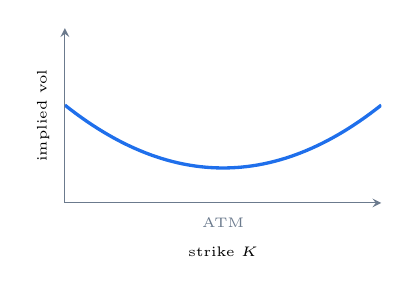
\begin{tikzpicture}
        \begin{axis}[width=5.6cm,height=3.8cm,axis lines=left,
            tick style={draw=none}, xlabel={\tiny strike $K$}, ylabel={\tiny implied vol},
            label style={font=\tiny}, ticklabel style={font=\tiny,color=muted},
            axis line style={draw=muted}, xmin=60,xmax=140,ymin=0.12,ymax=0.32,
            xtick={100}, xticklabels={ATM}, ytick=\empty, domain=60:140, samples=60]
          \addplot[accent, line width=1.2pt]{ 0.16 + 0.000045*(x-100)^2 };
        \end{axis}
      \end{tikzpicture}\\
      {\tiny\color{muted}out-of-the-money options cost \emph{more} vol}
    \end{column}
  \end{columns}
\end{frame}

%--- 16. Strategies: protective / covered -----------------------------------
\begin{frame}{Part IV — Strategies I: shaping a stock position}
  Options let you \emph{reshape} the payoff of a holding.
  \vspace{0.3em}
  \begin{columns}[T]
    \begin{column}{0.5\textwidth}
      \centering{\scriptsize\textbf{Protective Put} \;=\; long stock $+$ long put}\\[-0.1em]
      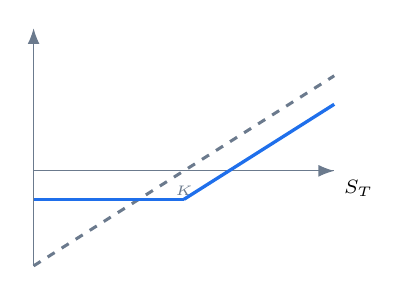
\begin{tikzpicture}
        \begin{axis}[payoffaxis, width=5.4cm, xlabel={$S_T$}, ymin=-2, ymax=3, xmin=0, xmax=4, xtick={2}, xticklabels={$K$}, ytick=\empty]
          \addplot[muted,dashed, domain=0:4]{x-2};              % stock
          \addplot[accent, line width=1.2pt, domain=0:2]{-0.6}; % floor
          \addplot[accent, line width=1.2pt, domain=2:4]{x-2-0.6};
          \draw[muted,dashed] (axis cs:0,0)--(axis cs:4,0);
        \end{axis}
      \end{tikzpicture}\\
      {\scriptsize insures the downside; you pay the premium}
    \end{column}
    \begin{column}{0.5\textwidth}
      \centering{\scriptsize\textbf{Covered Call} \;=\; long stock $+$ short call}\\[-0.1em]
      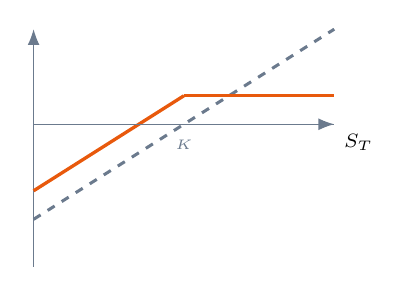
\begin{tikzpicture}
        \begin{axis}[payoffaxis, width=5.4cm, xlabel={$S_T$}, ymin=-3, ymax=2, xmin=0, xmax=4, xtick={2}, xticklabels={$K$}, ytick=\empty]
          \addplot[muted,dashed, domain=0:4]{x-2};              % stock
          \addplot[accent2, line width=1.2pt, domain=0:2]{x-2+0.6};
          \addplot[accent2, line width=1.2pt, domain=2:4]{0.6}; % capped
          \draw[muted,dashed] (axis cs:0,0)--(axis cs:4,0);
        \end{axis}
      \end{tikzpicture}\\
      {\scriptsize earns premium; caps the upside}
    \end{column}
  \end{columns}
  \vspace{0.3em}
  \keybox{Same underlying, two different risk profiles — you buy insurance, or you sell it.}
\end{frame}

%--- 17. Strategies: spreads ------------------------------------------------
\begin{frame}{Strategies II: spreads — a defined-risk directional bet}
  A \alert{vertical spread} combines two options of the same type and
  expiry but different strikes. It caps \emph{both} profit and loss and
  lowers the cost.
  \vspace{0.3em}
  \begin{columns}[c]
    \begin{column}{0.5\textwidth}
      \centering{\scriptsize\textbf{Bull Call Spread} \;=\; long call $K_1$ $+$ short call $K_2$}\\[-0.1em]
      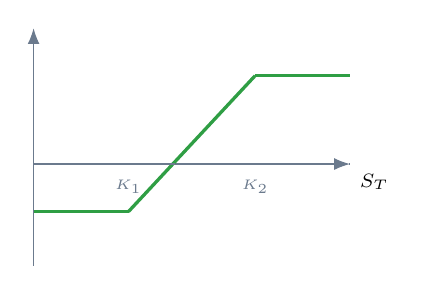
\begin{tikzpicture}
        \begin{axis}[payoffaxis, width=5.6cm, xlabel={$S_T$}, ymin=-1.5, ymax=2, xmin=0, xmax=5,
            xtick={1.5,3.5}, xticklabels={$K_1$,$K_2$}, ytick=\empty]
          \addplot[good, line width=1.2pt, domain=0:1.5]{-0.7};
          \addplot[good, line width=1.2pt, domain=1.5:3.5]{-0.7+(x-1.5)};
          \addplot[good, line width=1.2pt, domain=3.5:5]{1.3};
          \draw[muted,dashed] (axis cs:0,0)--(axis cs:5,0);
        \end{axis}
      \end{tikzpicture}
    \end{column}
    \begin{column}{0.5\textwidth}
      \begin{itemize}\small
        \item \textbf{Max loss} = net premium paid (floor).
        \item \textbf{Max gain} = $(K_2-K_1)-$ premium (ceiling).
        \item Cheaper than a bare call: you finance it by selling the upper strike.
        \item Mirror it with puts for a \textbf{bear put spread} — a defined-risk \emph{down} bet.
      \end{itemize}
    \end{column}
  \end{columns}
  \vspace{0.2em}
  \keybox{Spreads express a \emph{view with boundaries}: ``up, but only this far, and I'll risk only this much.''}
\end{frame}

%--- 18. Strategies: volatility ---------------------------------------------
\begin{frame}{Strategies III: trading volatility, not direction}
  A \alert{straddle} (long call $+$ long put, same strike) profits from a
  \emph{big move either way} — it is a pure bet that realised volatility
  will beat the implied volatility you paid.
  \vspace{0.2em}
  \begin{columns}[c]
    \begin{column}{0.46\textwidth}
      \centering{\scriptsize\textbf{Long Straddle}}\\[-0.1em]
      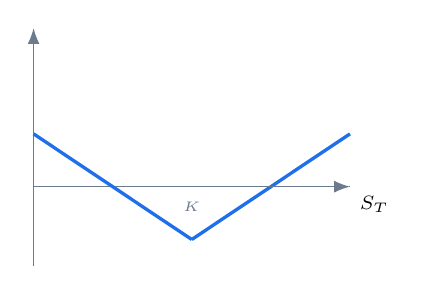
\begin{tikzpicture}
        \begin{axis}[payoffaxis, width=5.6cm, xlabel={$S_T$}, ymin=-1.5, ymax=3, xmin=0, xmax=4,
            xtick={2}, xticklabels={$K$}, ytick=\empty]
          \addplot[accent, line width=1.2pt, domain=0:2]{(2-x)-1};
          \addplot[accent, line width=1.2pt, domain=2:4]{(x-2)-1};
          \draw[muted,dashed] (axis cs:0,0)--(axis cs:4,0);
        \end{axis}
      \end{tikzpicture}
    \end{column}
    \begin{column}{0.54\textwidth}
      \begin{itemize}\small
        \item \textbf{Long} straddle: profit if $\und$ moves far from $\strike$; loss if it sits still (you bleed Theta). Long Gamma \& Vega.
        \item \textbf{Short} straddle: the opposite — earn premium if the market is calm, but open-ended risk if it jumps.
        \item A \textbf{strangle} uses OTM strikes: cheaper, needs a bigger move.
      \end{itemize}
    \end{column}
  \end{columns}
  \vspace{0.2em}
  \keybox{You can be right about \emph{volatility} while having no view on \emph{direction} at all.}
\end{frame}

%--- 19. Risk management ----------------------------------------------------
\begin{frame}{Managing risk with the Greeks}
  A trading book holds many positions. Its total risk is the \emph{aggregate}
  of Greeks — you manage the book by steering these numbers to target levels.
  \[
    \Delta_{\text{book}}=\sum_i \Delta_i,\quad
    \Gamma_{\text{book}}=\sum_i \Gamma_i,\quad
    \mathcal{V}_{\text{book}}=\sum_i \mathcal{V}_i,\ \dots
  \]
  \begin{columns}[T]
    \begin{column}{0.5\textwidth}
      \textbf{A typical workflow}
      \begin{enumerate}\small
        \item Neutralise unwanted \textbf{Delta} with the underlying.
        \item Cap \textbf{Gamma}/\textbf{Vega} with offsetting options.
        \item Watch \textbf{Theta} — the daily cost of being long convexity.
        \item Stress-test: ``what if $\und$ jumps $10\%$ and $\sigma$ doubles?''
      \end{enumerate}
    \end{column}
    \begin{column}{0.5\textwidth}
      \textbf{Broader tools}
      \begin{itemize}\small
        \item \textbf{Value-at-Risk (VaR):} a loss threshold breached only with probability $\alpha$.
        \item \textbf{Position limits} \& \textbf{stop-losses}.
        \item \textbf{Diversification} across underlyings and expiries.
        \item Respect \textbf{tail risk} — models understate extremes.
      \end{itemize}
    \end{column}
  \end{columns}
  \vspace{0.15em}
  \keybox{Options are the most precise instrument we have for \emph{sculpting} a risk profile — not just reducing risk, but choosing its exact shape.}
\end{frame}

%--- 20. Summary ------------------------------------------------------------
\begin{frame}{Key takeaways}
  \begin{columns}[T]
    \begin{column}{0.5\textwidth}
      \textbf{\color{accent}The ideas}
      \begin{itemize}\small
        \item Prices are \textbf{random}; volatility measures the risk.
        \item An \textbf{option} is a right, not an obligation — asymmetric payoff.
        \item Its value $=$ \textbf{intrinsic} $+$ \textbf{time value}, priced by \textbf{no-arbitrage} (Black--Scholes).
        \item The \textbf{Greeks} decompose that price into manageable risks.
      \end{itemize}
    \end{column}
    \begin{column}{0.5\textwidth}
      \textbf{\color{accent}The craft}
      \begin{itemize}\small
        \item \textbf{Delta-hedge} to isolate the bet you actually want.
        \item Trade \textbf{direction} (spreads) or \textbf{volatility} (straddles) deliberately.
        \item Long options: pay \textbf{Theta} for \textbf{Gamma/Vega}. Short: the reverse.
        \item Manage the \textbf{book} by its aggregate Greeks and its tails.
      \end{itemize}
    \end{column}
  \end{columns}
  \vfill
  \begin{center}
    {\color{accent}\rule{0.5\textwidth}{1pt}}\\[0.5em]
    \small\color{muted}Further reading: Hull, \emph{Options, Futures \& Other Derivatives}\;$\cdot$\;
    Natenberg, \emph{Option Volatility \& Pricing}
  \end{center}
\end{frame}

\end{document}
